%!Mode:: "TeX:UTF-8"
\documentclass{beamer}
\usepackage{xeCJK}
\usepackage{xcolor}
\usepackage{listings}
\usepackage{soul}
\usepackage{ulem}
\usepackage{url}
\usepackage{graphicx}

\setCJKmainfont{WenQuanYi Zen Hei}



%\setbeamertemplate{footline}[frame number]
%\setbeamertemplate{navigation symbols}{}
\usetheme{Madrid}
\begin{document}

\title{报告}
\author{王海霞}


\maketitle

%\begin{frame}
%    \frametitle{OUTLINE}
%    \tableofcontents
%\end{frame}

\begin{frame}
%\frametitle{}
    \begin{itemize}
        \item 写root脚本实现对GBBhabha事例寻迹和kalman的一些值的分析
            \begin{itemize}
                \item 分别采用高斯拟合和RooFit拟合,
                    找出动量随方位角的分布,$\sigma$随方位角的变化,
                    动量随$\theta$的变化,残差分布等。 
            \end{itemize}
        \item 将动量boost到质心系下看动量分辨
            \begin{itemize}
                \item 将动量boost到质心系下看动量分辨,
                    因为正负电子对撞时有22mrad的夹角,
                    这会导致在实验系下的动量随方位角变化,
                    为了得到正确的动量分辨,
                    必须把动量测量值转换到质心系下,
                    这样也可以检查刻度的效果。 
            \end{itemize}
        \item 用besvis.exe查看有问题的实例,找出原因
            \begin{itemize}
                \item 如填图时发现doca的值很大,很明显不符合实际,
                    通过FileFilterAlg过滤算法得到这些值对应的事例号和run号,
                    在事例显示器上发现这些点是重建出来的假径迹,
                    还有一些点没有在径迹上,原因正在找寻中。 
            \end{itemize}
    \end{itemize}
\end{frame}

\begin{frame}
    \frametitle{实验系下寻迹动量和kalman动量的比较}
    \begin{columns}
        \column{6.0cm}
        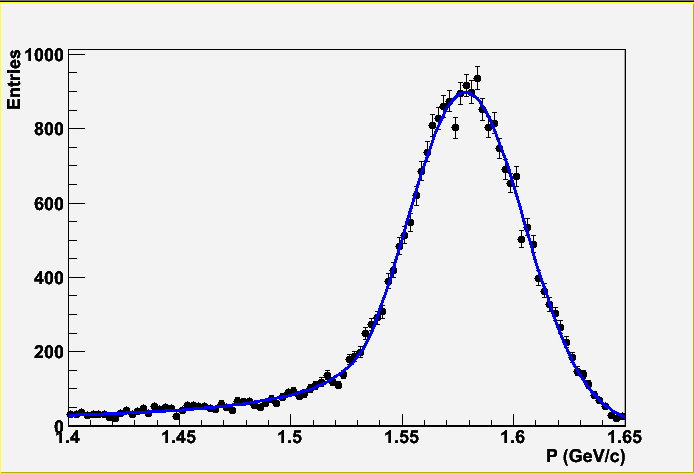
\includegraphics[width=6cm, keepaspectratio]{data/p.png}
        \column{6.0cm}
        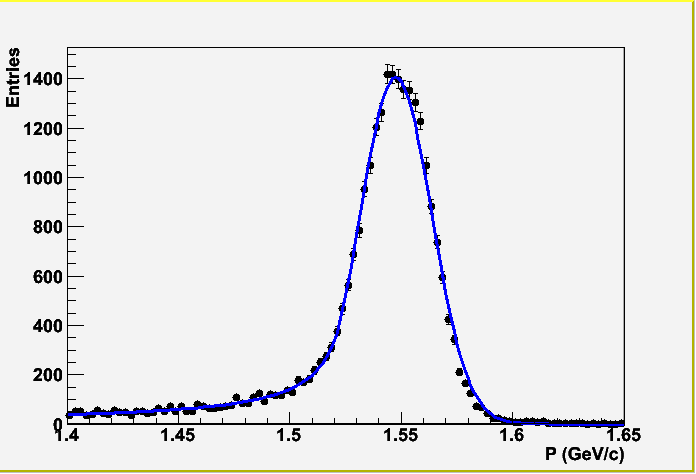
\includegraphics[width=6cm, keepaspectratio]{data/p_kal.png}
    \end{columns}
    \begin{itemize}
        \item kalman动量的RMS值更小,说明实验系下kalman动量离散程度小 
    \end{itemize}

\end{frame}


\begin{frame}
    \frametitle{质心系下寻迹动量和kalman动量的比较}
    \begin{columns}
        \column{6.0cm}
        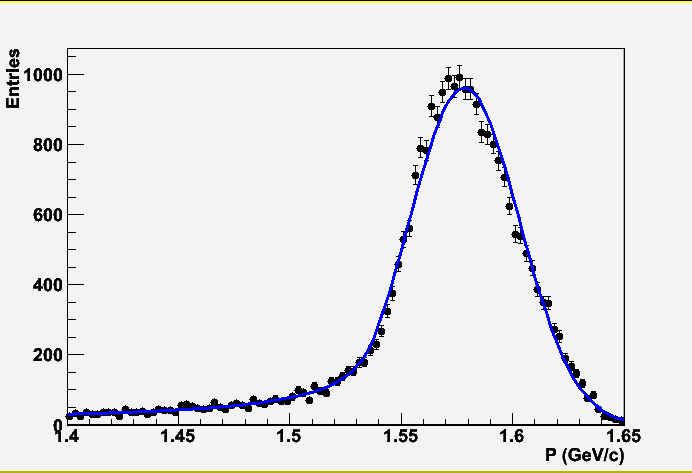
\includegraphics[width=6cm, keepaspectratio]{data/pcms.png}
        \column{6.0cm}
        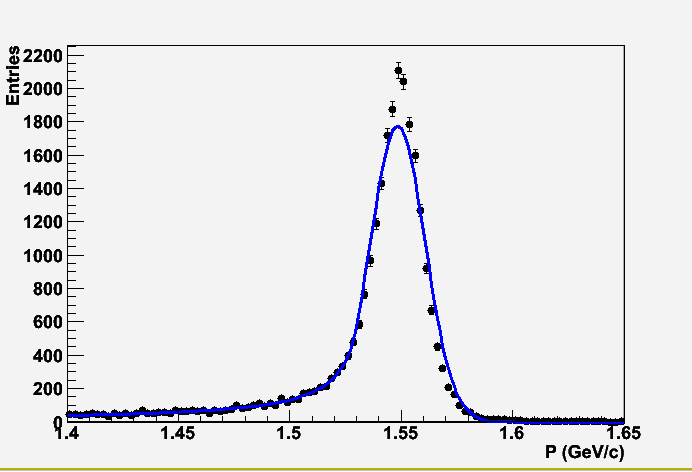
\includegraphics[width=6cm, keepaspectratio]{data/pcms_kal.png}
    \end{columns}
    \begin{itemize}
        \item kalman动量的RMS小,说明在质心系下kalman的动量的离散程度小
    \end{itemize}

\end{frame}


\begin{frame}
    \frametitle{实验系下和质心系下寻迹动量的比较}
    \begin{columns}
        \column{6.0cm}
        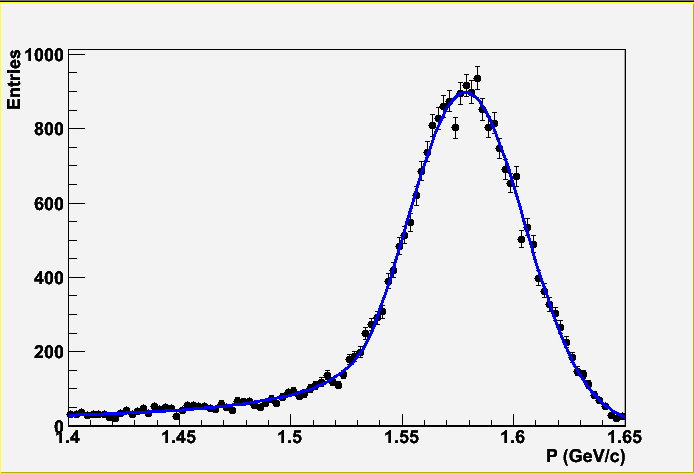
\includegraphics[width=6cm, keepaspectratio]{data/p.png}
        \column{6.0cm}
        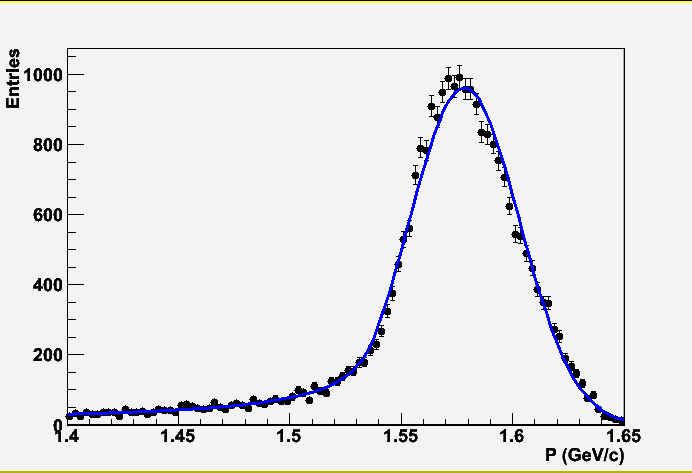
\includegraphics[width=6cm, keepaspectratio]{data/pcms.png}
    \end{columns}
    \begin{itemize}
        \item 

    \end{itemize}

\end{frame}


\begin{frame}
    \frametitle{实验系下和质心系下kalman动量的比较}
    \begin{columns}
        \column{6.0cm}
        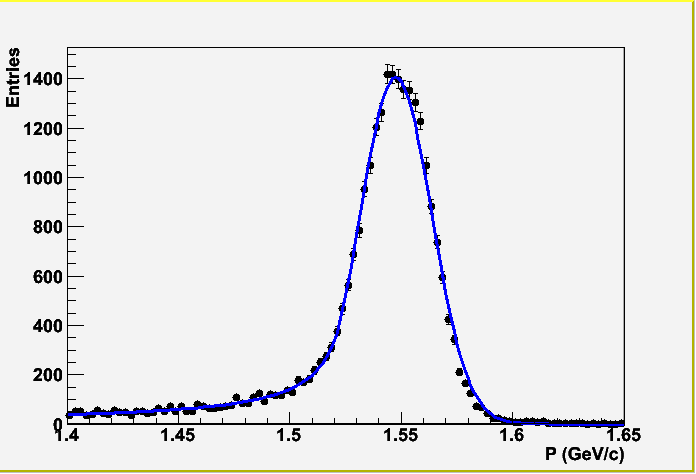
\includegraphics[width=6cm, keepaspectratio]{data/p_kal.png}
        \column{6.0cm}
        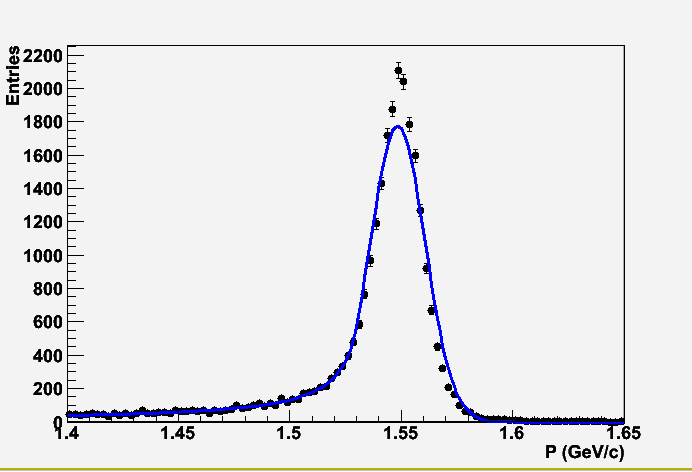
\includegraphics[width=6cm, keepaspectratio]{data/pcms_kal.png}
    \end{columns}
    \begin{itemize}
        \item 
    \end{itemize}

\end{frame}


\begin{frame}
    \frametitle{高斯拟合实验系和质心系下寻迹动量随方位角的分布}
    \begin{columns}
        \column{6.0cm}
        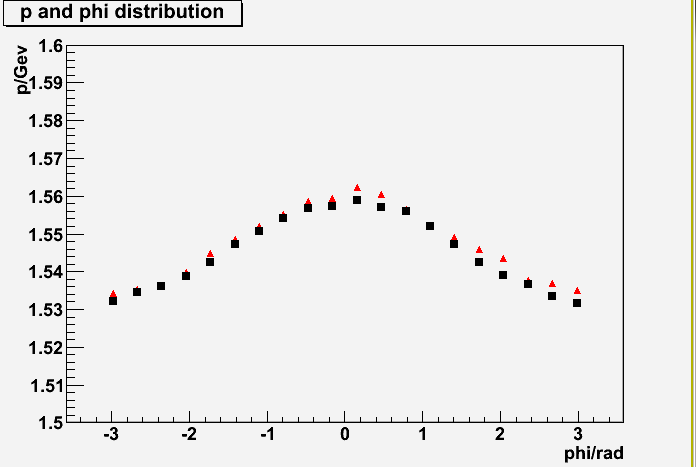
\includegraphics[width=6cm, keepaspectratio]{data/p_phi.png}
        \column{6.0cm}
        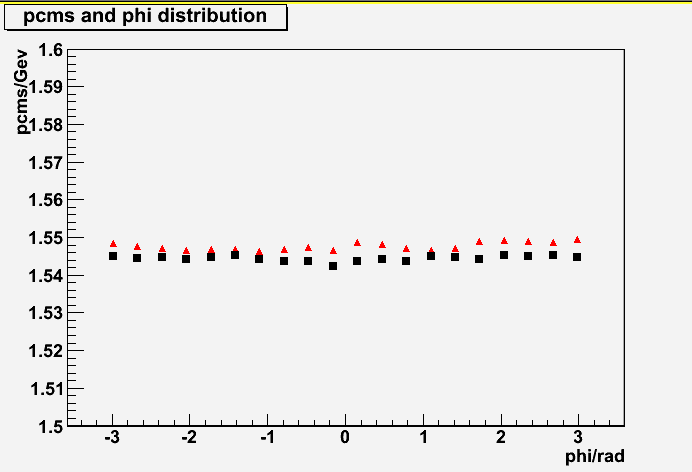
\includegraphics[width=6cm, keepaspectratio]{data/pcms_phi0.png}
    \end{columns}
    \begin{itemize}
        \item 
    \end{itemize}

\end{frame}


\begin{frame}
    \frametitle{高斯拟合实验系下和质心系下kalman动量随方位角的分布}
    \begin{columns}
        \column{6.0cm}
        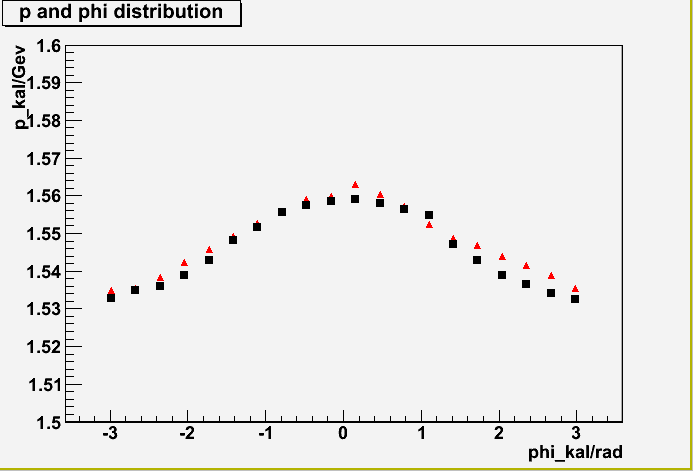
\includegraphics[width=6cm, keepaspectratio]{data/p_kal_phi_kal.png}
        \column{6.0cm}
        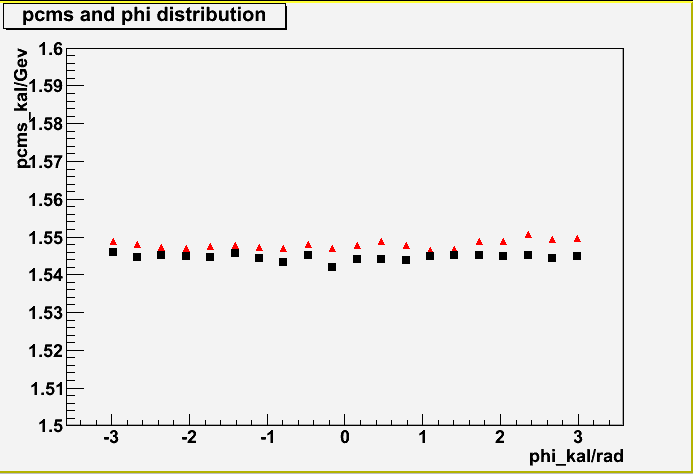
\includegraphics[width=6cm, keepaspectratio]{data/pcms_kal_phi_kal01.png}
    \end{columns}
    \begin{itemize}
        \item kalman动量分布峰位值随方位角的变化,
            实验系下是余弦分布,boost到质心系下后,
            动量峰位值随方位角分布接近水平直线分布,
            动量接近1.548Gev,并且正负电子的动量不一致,展宽了总动量分辨。
    \end{itemize}

\end{frame}

\begin{frame}
    \frametitle{高斯拟合和RooFit拟合质心系下kalman动量峰位值随方位角的分布的对比}
    \begin{columns}
        \column{6.0cm}
        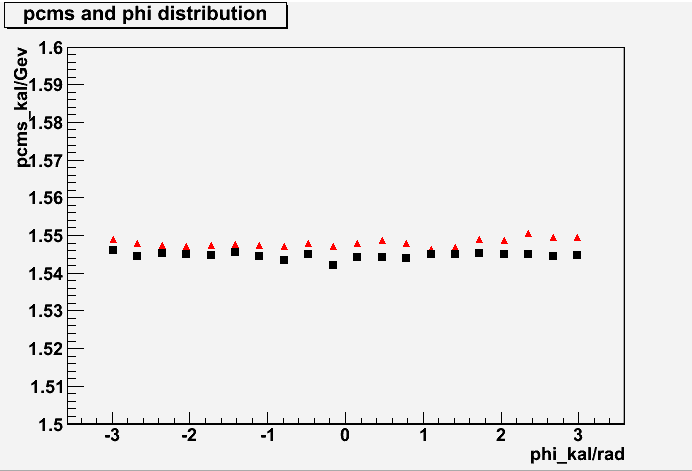
\includegraphics[width=6cm, keepaspectratio]{data/mean0.png}
        \column{6.0cm}
        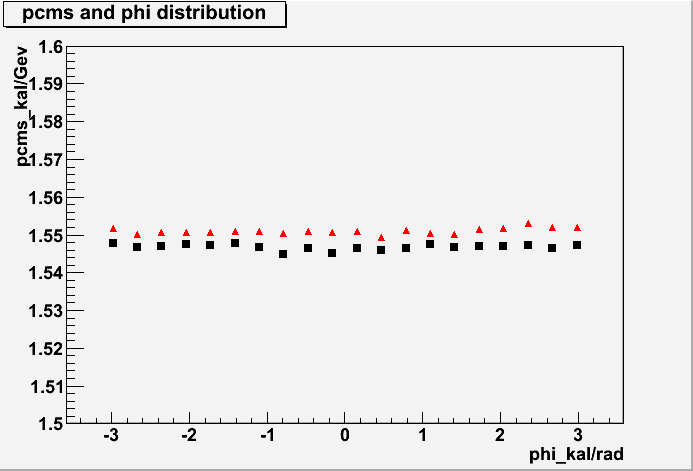
\includegraphics[width=6cm, keepaspectratio]{data/mean.png}
    \end{columns}
    \begin{itemize}
        \item 实际上动量分布是高斯不对称的,用RooFit拟合更好。
            两种拟合下下动量峰位值随方位角分布相差不大。
    \end{itemize}

\end{frame}

\begin{frame}
    \frametitle{高斯拟合和RooFit拟合质心系下kalman动量的$\sigma$值随方位角的分布的对比}
    \begin{columns}
        \column{6.0cm}
        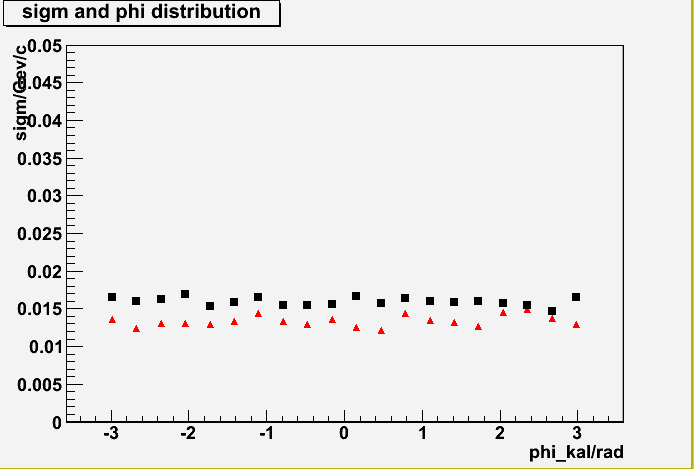
\includegraphics[width=6cm, keepaspectratio]{data/sigm0.png}
        \column{6.0cm}
        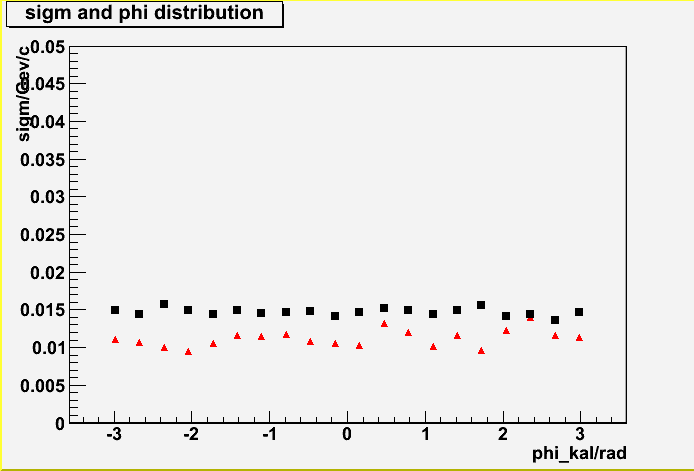
\includegraphics[width=6cm, keepaspectratio]{data/sigm.png}
    \end{columns}
    \begin{itemize}
        \item 两种拟合下$\sigma$随方位角分布相差不大,$\sigma$大约等于15.0Mev/c。
    \end{itemize}

\end{frame}

\begin{frame}
    \frametitle{crystall ball拟合实验系下下kalman动量峰位值和的$\sigma$值随方位角的分布的对比}
    \begin{columns}
        \column{6.0cm}
        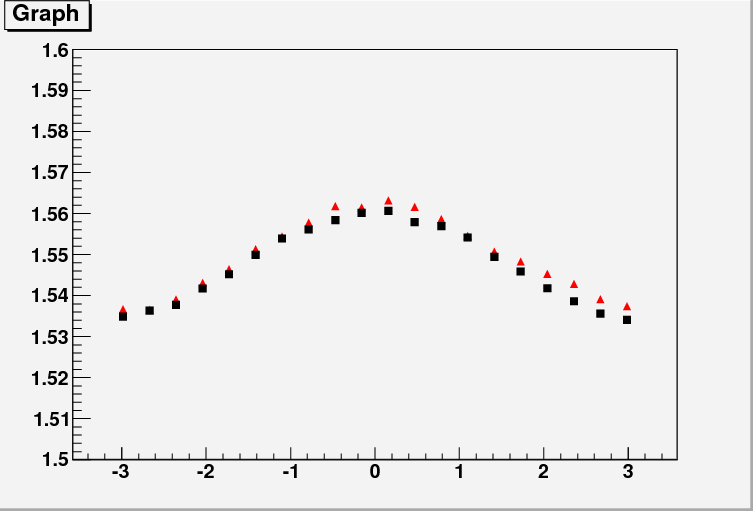
\includegraphics[width=6cm, keepaspectratio]{data/pmean_phi.png}
        \column{6.0cm}
        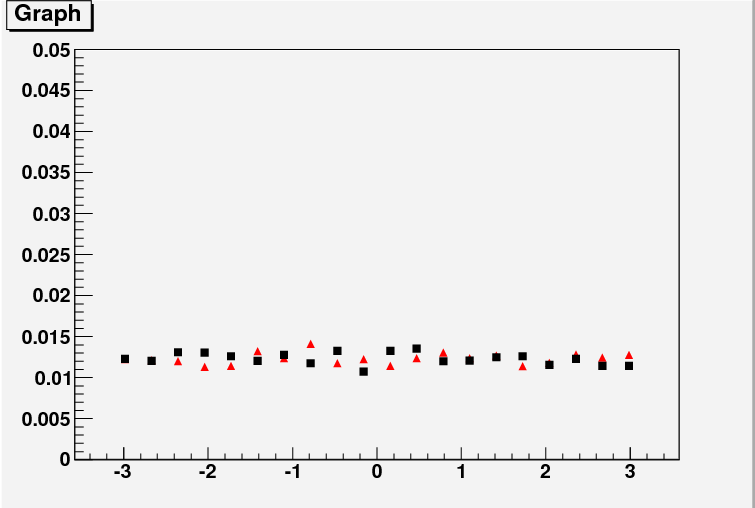
\includegraphics[width=6cm, keepaspectratio]{data/psigm_phi.png}
    \end{columns}
    \begin{itemize}
        \item 
    \end{itemize}

\end{frame}


\begin{frame}
    \frametitle{crystall ball拟合质心系下kalman动量峰位值和的$\sigma$值随方位角的分布的对比}
    \begin{columns}
        \column{6.0cm}
        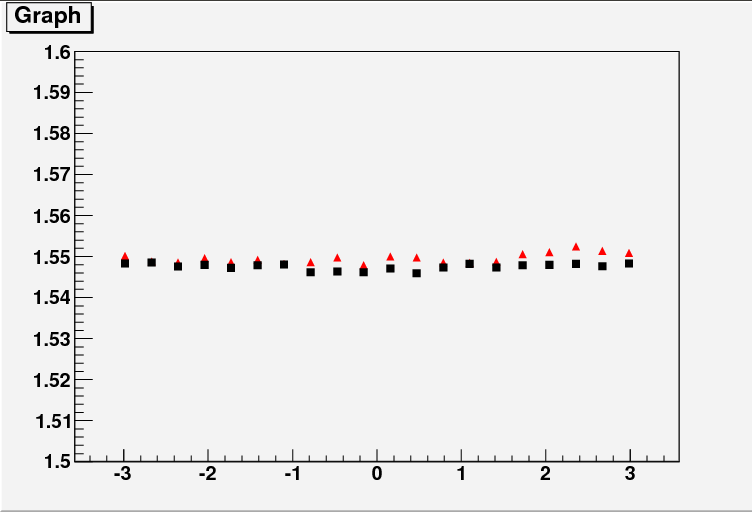
\includegraphics[width=6cm, keepaspectratio]{data/pcmsmean_phi.png}
        \column{6.0cm}
        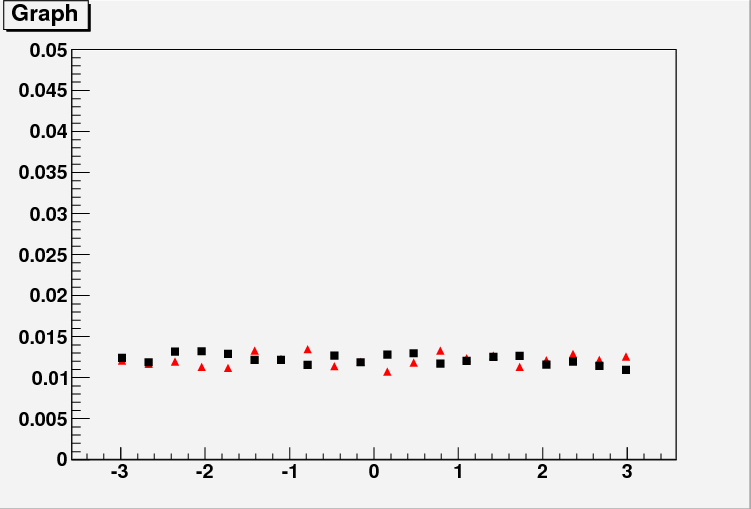
\includegraphics[width=6cm, keepaspectratio]{data/pcmssigm_phi.png}
    \end{columns}
    \begin{itemize}
        \item 
    \end{itemize}

\end{frame}



\begin{frame}
    \frametitle{crystall ball拟合实验系下kalman动量峰位值和的$\sigma$值随cos$\theta$的分布的对比}
    \begin{columns}
        \column{6.0cm}
        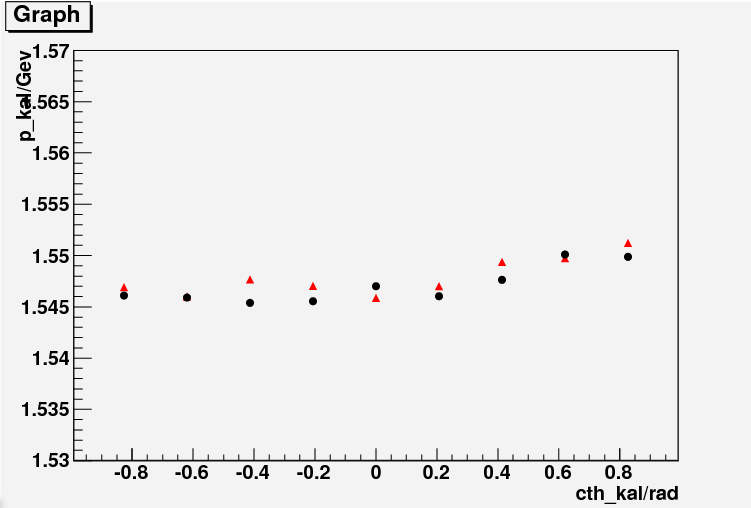
\includegraphics[width=6cm, keepaspectratio]{data/pmean_cth.png}
        \column{6.0cm}
        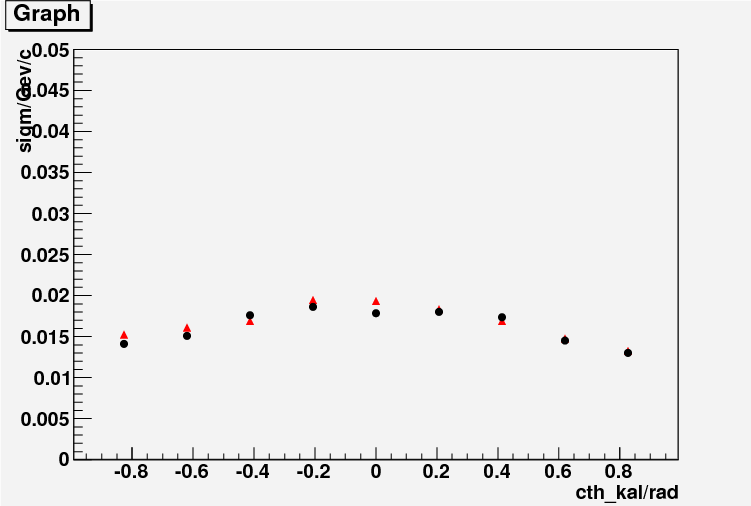
\includegraphics[width=6cm, keepaspectratio]{data/psigm_cth.png}
    \end{columns}
    \begin{itemize}
        \item 
    \end{itemize}

\end{frame}

\begin{frame}
    \frametitle{crystall ball拟合质心系下kalman动量峰位值和的$\sigma$值随cos$\theta$的分布的对比}
    \begin{columns}
        \column{6.0cm}
        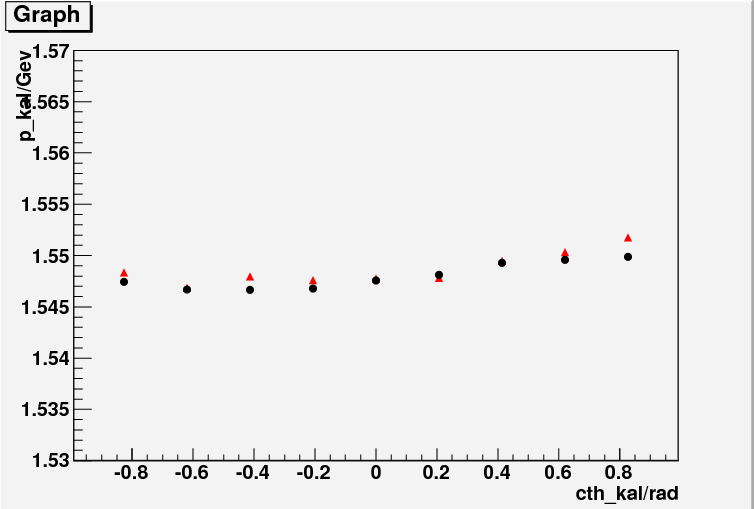
\includegraphics[width=6cm, keepaspectratio]{data/pcmsmean_cth.png}
        \column{6.0cm}
        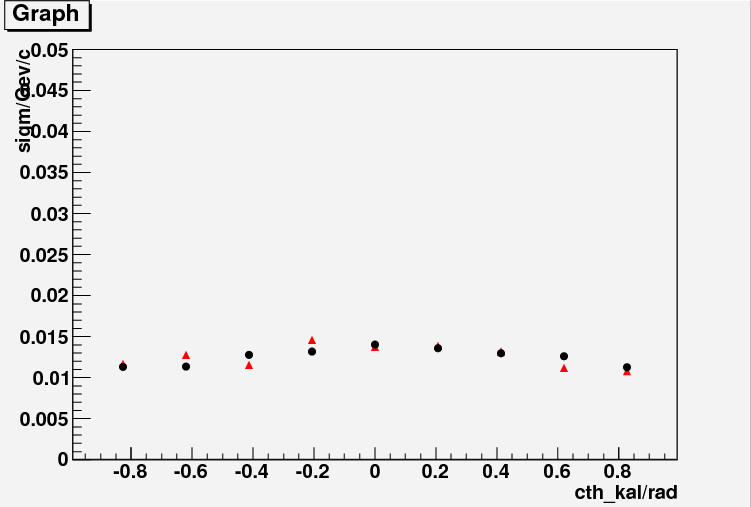
\includegraphics[width=6cm, keepaspectratio]{data/pcmssigm_cth.png}
    \end{columns}
    \begin{itemize}
        \item 
    \end{itemize}

\end{frame}


\section*{end}
\begin{frame}
    \begin{center}
        \Huge Thank you
    \end{center}
\end{frame}



\end{document}
